\documentclass[letterpaper,12pt]{article}
\usepackage{array}
\usepackage{geometry}
\geometry{letterpaper,tmargin=1in,bmargin=1in,lmargin=1.25in,rmargin=1.25in}
%\renewcommand\headrulewidth{0pt}
%\renewcommand\footrulewidth{0pt}
\usepackage{amsmath}
\usepackage{amssymb}
\usepackage{amsthm}
\usepackage{enumerate}
%\usepackage{harvard}
%\usepackage{setspace}
\usepackage{float,color}
\usepackage[pdftex]{graphicx}
\usepackage{hyperref}
\hypersetup{colorlinks,linkcolor=red,urlcolor=blue}
\theoremstyle{definition}
\newtheorem{theorem}{Theorem}
\newtheorem{acknowledgement}[theorem]{Acknowledgement}
\newtheorem{algorithm}[theorem]{Algorithm}
\newtheorem{axiom}[theorem]{Axiom}
\newtheorem{case}[theorem]{Case}
\newtheorem{claim}[theorem]{Claim}
\newtheorem{conclusion}[theorem]{Conclusion}
\newtheorem{condition}[theorem]{Condition}
\newtheorem{conjecture}[theorem]{Conjecture}
\newtheorem{corollary}[theorem]{Corollary}
\newtheorem{criterion}[theorem]{Criterion}
\newtheorem{definition}[theorem]{Definition}
\newtheorem{derivation}{Derivation} % Number derivations on their own
\newtheorem{example}[theorem]{Example}
\newtheorem{exercise}[theorem]{Exercise}
\newtheorem{lemma}[theorem]{Lemma}
\newtheorem{notation}[theorem]{Notation}
\newtheorem{problem}[theorem]{Problem}
\newtheorem{proposition}{Proposition} % Number propositions on their own
\newtheorem{remark}[theorem]{Remark}
\newtheorem{solution}[theorem]{Solution}
\newtheorem{summary}[theorem]{Summary}
%\numberwithin{equation}{section}
\bibliographystyle{aer}
\newcommand\ve{\varepsilon}
\newcommand\boldline{\arrayrulewidth{1pt}\hline}


\begin{document}

\begin{flushleft}
   \textbf{\large{Problem Set \#2}} \\
   MACS 40000, Dr. Evans \\
   Alexandre Sollaci
\end{flushleft}

\vspace{5mm}

\noindent\begin{enumerate}
   \item \textbf{Checking Feasibility in the steady state}
	\begin{enumerate}[(a)]
		\item With \texttt{bvec\_guess = np.array([1., 1.2])}, the \texttt{feasible} function returns:
		 \texttt{b\_cnstr = array([ True, False], dtype=bool), c\_cnstr = array([ True, False, False], dtype=bool), K\_cnstr = False}. \linebreak
		 Hence, the non-negativity constraint for consumption is violated for one period old individuals. Because of that, the first element of \texttt{b\_cnstr} is also \texttt{True}.
		 
		 \item In this case, none of the constraints are violated: \hfill \hfill \linebreak
		 \texttt{b\_cnstr = array([False, False], dtype=bool), c\_cnstr = array([False, False, False], dtype=bool), K\_cnstr = False}.
		 
		\item As in part (b), none of the constraints are violated for this initial guess. 
		 
	\end{enumerate}
		
		
   \item \textbf{Solve for the steady state equilibrium}
   \begin{enumerate}[(a)]
   \item The function \texttt{get\_SS} produces the following output:
   
   \begin{verbatim}
   	{'C_ss': 0.63290067293958485,
 	'EulErr_ss': array([ -3.33066907e-16,  -5.55111512e-16]),
 	'K_ss': 0.077723625753163231,
 	'RCerr_ss': 1.5265566588595902e-16,
 	'Y_ss': 0.68276037886023921,
 	'b_ss': array([ 0.01931253,  0.0584111 ]),
 	'c_ss': array([ 0.18241213,  0.20961468,  0.24087387]),
	  'r_ss': 2.4330623391270851,
	  'ss_time': 0.001122023435527808,
 	'w_ss': 0.20172465739052517}
	\end{verbatim}    
Figure 1 shows the distribution of consumption and savings in steady state:
	
	\item When $\beta$ increases to 0.55, the new steady state is characterized by:
	
	\begin{verbatim}
		    {'C_ss': 0.6912842903551415,
 	'EulErr_ss': array([  2.22044605e-16,  -3.33066907e-16]),
 	'K_ss': 0.10504237022597476,
 	'RCerr_ss': 1.3877787807814457e-17,
 	'Y_ss': 0.75866897085510432,
 	'b_ss': array([ 0.02817692,  0.07686545]),
 	'c_ss': array([ 0.19597528,  0.22861594,  0.26669307]),
	  'r_ss': 1.8863765057190751,
 	'ss_time': 0.0009647841470723506,
 	'w_ss': 0.22415219593446262}
 
	\end{verbatim}
	As evidenced by the values displayed above, both consumption and savings increase, interest rate decreases and wage increases. The intuition is that a higher $\beta$ means that individuals are more patient. This means that they save more for old age. In equilibrium, this will decrease the interest rate (since the supply of investment has exogenously increased), increasing the usage of capital. Since firms use more capital, the marginal product of labor increases, and thus wages increase as well. Consumption in this case also increases as total production increases as a result of the firm using more capital.
	\end{enumerate}
	
	\item \textbf{Solve for the non-steady-state equilibrium time path}
	
	In this question, I use $T = 50$ and $\xi = 0.8$.
	\begin{enumerate}[(a)]
		\item Figure 2 shows the time path of capital to steady state. Similarly, figures 3 and 4 show the time path of wages and interest rate to steady state.
		\item With the parameters I used, it took 7 periods for $K$ to get within 0.0001 of the steady state capital stock.
	\end{enumerate}		
	
\end{enumerate}
\clearpage

\section*{Figures}

\begin{figure}[h!]
\centering
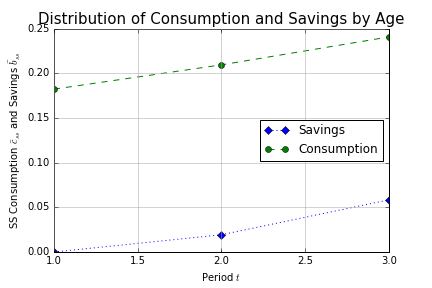
\includegraphics[scale=1]{figures/cons_savings_dist}
\caption{Consumption and savings in steady state.}
\end{figure}

\begin{figure}[h!]
\centering
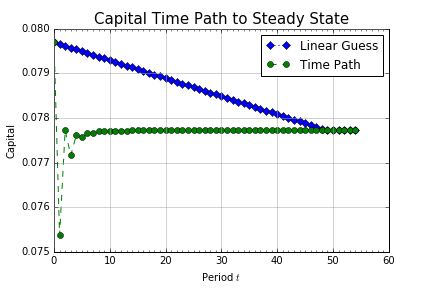
\includegraphics[scale=1]{figures/time_path_K}
\caption{Time path of capital to steady state.}
\end{figure}

\begin{figure}[h!]
\centering
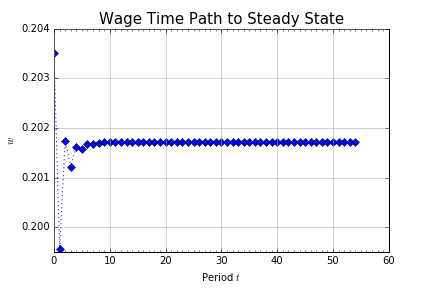
\includegraphics[scale=1]{figures/time_path_w}
\caption{Time path of wage to steady state.}
\end{figure}

\begin{figure}[h!]
\centering
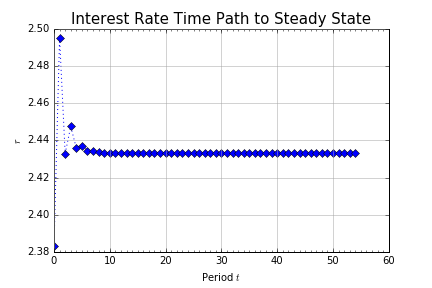
\includegraphics[scale=1]{figures/time_path_r}
\caption{Time path of interest rate to steady state.}
\end{figure}

\end{document}





